%%%%%%%%%%%%%%%%%%%%%%%%%%%%%%%%%%%%%%%%%%%%%%%%%%%%%%%%%%%%%%%%%%%%%%%%%%%%%%%
% Chapter 3: Gestión de la configuración
%%%%%%%%%%%%%%%%%%%%%%%%%%%%%%%%%%%%%%%%%%%%%%%%%%%%%%%%%%%%%%%%%%%%%%%%%%%%%%%

\section{PaaS}\label{cap.3.1}

En el capítulo de introducción~\ref{chapter:intro} se explicó los cambios en la elección del entorno de producción, así como su estudio. En este capítulo se explicará los dos entornos de producción escogidos, cómo funcionan y se configuran. \\

Antes de empezar debe quedar claro los modelos de servicios que ofrecen las nubes. Las empresas ofertan distintos servicios y prestaciones, de los cuales destacan:
\begin{itemize}
	\item \textbf{SaaS:} Software como servicio. Se trata de cualquier servicio basado en la web. En este tipo de servicios accedemos normalmente a través del navegador sin atender al software. Todo el desarrollo, mantenimiento, actualizaciones, copias de seguridad es responsabilidad del proveedor. Son ejemplos conocidos \emph{Google docs, Hotmail o Dropbox.}
	\item \textbf{PaaS:} Plataforma como servicio, es una encapsulación del entorno de desarrollo y un conjunto de módulos con el fin de proporcionar una funcionalidad que se traduce como servicio. En este modelo de servicio al usuario se le ofrece la plataforma de desarrollo y las herramientas de programación por lo que puede desarrollar aplicaciones propias y controlar la aplicación, pero no controla la infraestructura. Por ejemplo, \emph{Heroku, Google App Engine o Windows Azure}. 
	\item \textbf{IaaS:} Infraestructura como servicio. Tendremos más control que con PaaS, lo que implica la gestión de la infraestructura. Es un medio de entregar almacenamiento básico y capacidades de cómputo como servicios estandarizados en la red. Servidores, sistemas de almacenamiento, conexiones, enrutadores, y otros sistemas se concentran para manejar tipos específicos de cargas de trabajo. Algunos ejemplos son: \emph{Amazon Web Services, Google Cloud Storage y VMware}. 
\end{itemize}

Normalmente, para interactuar con la PaaS elegida, el proveedor proporciona una herramienta. Esta cambia en función de la nube elegida, pero su funcionamiento y opciones son similares: descargar la aplicación de un determinado repositorio y hacerla correr en la nube a modo de producción. Además ofrecen distintos servicios o módulos, normalmente de pago. En Heroku se conoce como \emph{dynos} y en OpenShift se llama \emph{cartridge}. Éstos pueden ser la base de datos con la que interactuará la aplicación, mejoras en el equipo servidor (nube de producción) como mayor capacidad de disco, memoria RAM, CPU, sistema dedicado, incluso aumentar el ancho de banda para atender más peticiones.

\begin{figure}[H]
	\centering
	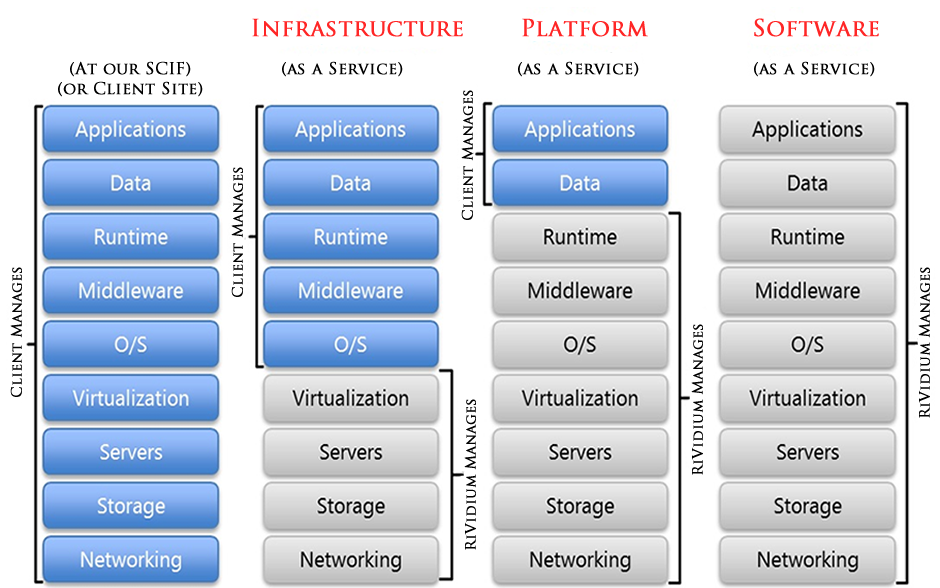
\includegraphics[width=12cm]{./images/cloud-models.png}
	\caption{Modelos de nubes} \label{fig:cloud-models}
\end{figure}

\vspace*{0.2in}
\section{Heroku}\label{cap.3.2}

Se trata de una plataforma de aplicaciones cloud que permite construir y desplegar aplicaciones web. Soporta distintos lenguajes y frameworks. Para poder usar esta plataforma lo primero es registrarse y acceder a la misma. Desde la pantallas de \emph{dashboard} podremos gestionar las aplicaciones o bien mediante los comandos de su herramienta (\href{https://devcenter.heroku.com/start}{\emph{Heroku Toolbelt}}). Existen tres formas de configurar nuestra aplicación en Heroku.
\begin{itemize}
	\item Desde el \textbf{dashboard}: Desde esta pantalla seleccionamos la app deseada y encontramos un menu con una serie de opciones que nos permiten gestionar la aplicación en la nube: añadir add-ons, activar \emph{dynos}, seleccionar repositorio, información como métricas y actividad del servidor, permiso de acceso a la app y la configuración propia de la app (variables, dominio, etc.).
	\item Mediante \textbf{Heroku Toolbelt}: Este comando (\$ heroku COMMAND) tiene múltiples opciones que permiten interactuar con la consola desde consola. Subir app, configurar la bbdd y variables, comprobar logs del servidor, etc. En resumen, las opciones que nos proporciona el \emph{dashboard} en el navegador, pero desde consola. Ejecute \$ heroku -h para acceder a la ayuda y opciones.
	\item A través de \textbf{archivos de configración}: Esta opción afecta más a la configuración de la propia aplicación. Desde aquí podemos crear variables, base de datos y otros, sin embargo, no se gestionan los dynos o add-ons pero sí usarlos o interactuar con ellos si están creados.
\end{itemize}

\vspace*{0.2in}
\section{OpenShift}\label{cap.3.3}
Es otra PaaS similar a la anterior, pero montada en Linux Red Hat. Permite desarrollar rápidamente, hosting y la escalabilidad de aplicaciones en entornos de la nube. Al contrario que Heroku, en la versión \emph{free} permite crear hasta tres aplicaciones (y la primera cinco), sin embargo, aunque Heroku solo permite postgresql en esta versión, OpenShift permite escoger entre MongoDB, MySQL y PostgreSQL. Para \textbf{ChefManagement}, hemos tenido que adaptarnos al cuello de botella de Heroku en cuanto bbdd y trabajaremos con postgres en ambas plataformas. \\

Aunque OpenShift no dispone de tantas opciones de configuración en su \emph{dashboard} si que permite crear añadir \emph{cartridges} inclusos creados por nosotros mismos. Por ejemplo, un \href{https://github.com/openshift-cartridges/jruby-cartridge}{cartucho} para hacer funcionar Jruby en OpenShift. \\

En cuanto a la \href{https://developers.openshift.com/en/managing-client-tools.html}{herramienta del cliente} permite la gestión con la nube de igual forma que con la herramienta de Heroku. Sin embargo, en esta nube, no se puede añadir ni modificar variables. La nube almacena la configuración por defecto en caso de que la proporcionada no sea válida. En todo caso habría que usar su herramienta o archivos de configuración. \\

Los archivos de configuración son muy útles si no queremos usar las variables por defecto que proporciona la nube. Hay dos formas de editar estos archivos, mediante la herramienta cliente o bien editando manualmente estos \href{https://blog.openshift.com/netsource-partners-shows-the-benefits-of-custom-environment-variables-on-openshift/}{archivos de configuración}.
